
%%%%%%%%%%%%%%%%%%%%%
\section{Chute libre}
%%%%%%%%%%%%%%%%%%%%%
%
\subsection{Définition}

On lache une balle. On observe que celle-ci se met en mouvement, se dirige vers le bas, puis frappe le sol. Cette succession d'évènements constitue un phénomène : le phénomène de la chute libre.
\begin{center}

%%%%%%%%%%%%%%%%%%%%%        PERSONNAGE AU BORD D'UNE MARE
%  DÉFINITIONS

\tikzset{
  feuillage/.style = {decoration={random steps, segment length=0.4mm}, decorate},
  tronc/.style   = {decoration={random steps, segment length=2mm, amplitude=0.2mm}, decorate}}

\tikzset{  arbre/.pic={ \foreach \w/\f in {0.3/30,0.2/50,0.1/70} { \fill [brown!\f!black, tronc] (-\w/2,0) rectangle +(\w,3); } \foreach \n/\f in {1.4/40,1.2/50,1/60,0.8/70,0.6/80,0.4/90} { \fill [green!\f!black, feuillage](0,3) ellipse (\n/1.5 and \n); }}}

\tikzset{  personnage/.pic={ { \fill [black] (0,0)ellipse(0.25 and 0.55); } 
  { \fill [black](0,0.75)circle(0.2); }
    % jambe et pieds
  {\fill [rounded corners=2pt] (0.1,-0.3)rectangle(-0.1,-1.5);}
  {\fill [rounded corners=2pt] (0.3,-1.4)rectangle(-0.1,-1.5);}
    % bras
  {\fill [rounded corners=2pt, rotate=-15] (-0.1,0.42)rectangle(0.5,0.29);}
  {\fill [rounded corners=2pt] (0.44,0.17)rectangle(1,0.29);}}}

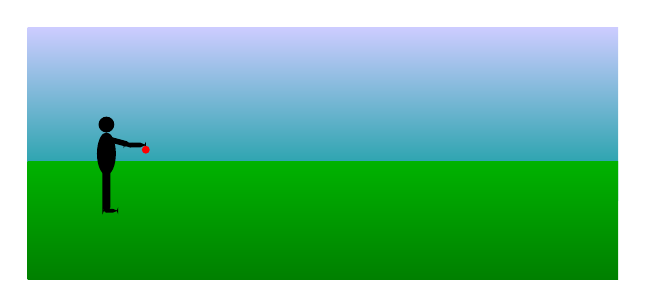
\begin{tikzpicture}%[scale=0.5]
    %  Ciel
  \shade[bottom color=cyan!60!black, top color=blue!20!white] (0,0) rectangle (7.5,2.2);
    %  Sol
  \shade[bottom color=green!50!black, top color=green!70!black] (0,0.5) rectangle (7.5,-1);
    %  Mare
 % \shade[bottom color=blue!50!white, top color=cyan!60!black] (3.7,-0.15) ellipse (2.5 and 0.3);
    %  Arbre
 % \pic at (2,2)    {arbre};

    %  Personnage
  \begin{scope}[xshift=1 cm,yshift=0.6 cm]
    % corps et tête
 \fill [black] (0,0)ellipse(0.12 and 0.27);
 \fill [black](0,0.37)circle(0.1);
    % jambe et pieds
 \fill [rounded corners=2pt] (0.05,-0.15)rectangle(-0.05,-0.75);
 \fill [rounded corners=2pt] (0.15,-0.7)rectangle(-0.05,-0.75);
    % bras
 \fill [rounded corners=2pt, rotate=-15] (-0.1,0.22)rectangle(0.28,0.15);
 \fill [rounded corners=2pt] (0.22,0.08)rectangle(0.5,0.14);
   % Balle
 \fill[red] (0.5,0.05) circle(0.05);
  \end{scope}

\end{tikzpicture}

%%%%%%%%%%%%%%%%%%%%%%%%%%%%%%%%%%%%%%%%%%%%%%%%%%%%%%%%%%%%%%%%%%%%%%%%%%%%%%%%

\end{center}

\subsection{Paradigmes}

Il existe plusieurs paradigmes qui tente de donner une explication rationnelle à ce phénomène. Pour aristote, la balle constituée de matière terrestre souhaite rejoindre le lieu de la matière terrestre qui est le bas. Pour Newton, la force gravitationnelle entre la Terre et la balle provoque la mise en mouvement de la balle. Pour Lagrange et Hamilton, l'énergie potentielle de gravitation de la balle se convertie en énergie cinétique. 


L'énergie potentielle est relié à la position, l'énergie cinétique est relié au mouvement, à la vitesse.

%\begin{minipage}[c]{.45\linewidth}
\begin{center}
Vision "Force de Gravitation"
\end{center}
La Terre exerce une force de gravitation $\overrightarrow{F}_{T/B}$ sur la balle $B$
%\setlength{\unitlength}{1cm}
\begin{center}

%%%%%%%%%%%%%%%%%%%%%        PERSONNAGE AU BORD D'UNE MARE
%  DÉFINITIONS

\tikzset{
  feuillage/.style = {decoration={random steps, segment length=0.4mm}, decorate},
  tronc/.style   = {decoration={random steps, segment length=2mm, amplitude=0.2mm}, decorate}}

\tikzset{  arbre/.pic={ \foreach \w/\f in {0.3/30,0.2/50,0.1/70} { \fill [brown!\f!black, tronc] (-\w/2,0) rectangle +(\w,3); } \foreach \n/\f in {1.4/40,1.2/50,1/60,0.8/70,0.6/80,0.4/90} { \fill [green!\f!black, feuillage](0,3) ellipse (\n/1.5 and \n); }}}

\tikzset{  personnage/.pic={ { \fill [black] (0,0)ellipse(0.25 and 0.55); } 
  { \fill [black](0,0.75)circle(0.2); }
    % jambe et pieds
  {\fill [rounded corners=2pt] (0.1,-0.3)rectangle(-0.1,-1.5);}
  {\fill [rounded corners=2pt] (0.3,-1.4)rectangle(-0.1,-1.5);}
    % bras
  {\fill [rounded corners=2pt, rotate=-15] (-0.1,0.42)rectangle(0.5,0.29);}
  {\fill [rounded corners=2pt] (0.44,0.17)rectangle(1,0.29);}}}

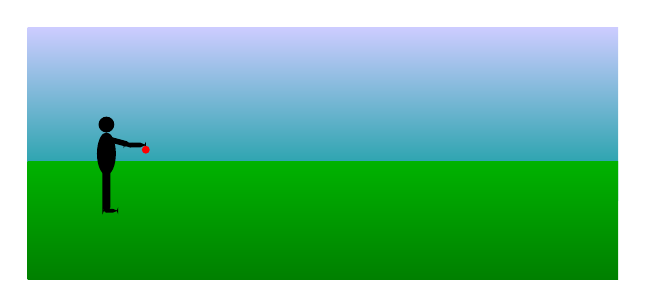
\begin{tikzpicture}%[scale=0.5]
    %  Ciel
  \shade[bottom color=cyan!60!black, top color=blue!20!white] (0,0) rectangle (7.5,2.2);
    %  Sol
  \shade[bottom color=green!50!black, top color=green!70!black] (0,0.5) rectangle (7.5,-1);
    %  Mare
 % \shade[bottom color=blue!50!white, top color=cyan!60!black] (3.7,-0.15) ellipse (2.5 and 0.3);
    %  Arbre
 % \pic at (2,2)    {arbre};

    %  Personnage
  \begin{scope}[xshift=1 cm,yshift=0.6 cm]
    % corps et tête
 \fill [black] (0,0)ellipse(0.12 and 0.27);
 \fill [black](0,0.37)circle(0.1);
    % jambe et pieds
 \fill [rounded corners=2pt] (0.05,-0.15)rectangle(-0.05,-0.75);
 \fill [rounded corners=2pt] (0.15,-0.7)rectangle(-0.05,-0.75);
    % bras
 \fill [rounded corners=2pt, rotate=-15] (-0.1,0.22)rectangle(0.28,0.15);
 \fill [rounded corners=2pt] (0.22,0.08)rectangle(0.5,0.14);
   % Balle
 \fill[red] (0.5,0.05) circle(0.05);
  \end{scope}

\end{tikzpicture}

%%%%%%%%%%%%%%%%%%%%%%%%%%%%%%%%%%%%%%%%%%%%%%%%%%%%%%%%%%%%%%%%%%%%%%%%%%%%%%%%

\end{center}
%\end{minipage}
%\hfill
%\begin{minipage}[c]{.45\linewidth}
\begin{center}
Vision "Énergétique"
\end{center}
La balle possède une énergie potentielle de gravitation lié à son altitude, au cours de sa chute, elle acquiert une énergie cinétique lié à sa vitesse. Au cours de la chutte, l'énergie potentielle est convertie en énergie cinétique. L'énergie totale, reste constante.
\begin{center}
%
%%%%%%%%%%%%%%%%%%%%%        PERSONNAGE AU BORD D'UNE MARE
%  DÉFINITIONS

\tikzset{
  feuillage/.style = {decoration={random steps, segment length=0.4mm}, decorate},
  tronc/.style   = {decoration={random steps, segment length=2mm, amplitude=0.2mm}, decorate}}

\tikzset{  arbre/.pic={ \foreach \w/\f in {0.3/30,0.2/50,0.1/70} { \fill [brown!\f!black, tronc] (-\w/2,0) rectangle +(\w,3); } \foreach \n/\f in {1.4/40,1.2/50,1/60,0.8/70,0.6/80,0.4/90} { \fill [green!\f!black, feuillage](0,3) ellipse (\n/1.5 and \n); }}}

\tikzset{  personnage/.pic={ { \fill [black] (0,0)ellipse(0.25 and 0.55); } 
  { \fill [black](0,0.75)circle(0.2); }
    % jambe et pieds
  {\fill [rounded corners=2pt] (0.1,-0.3)rectangle(-0.1,-1.5);}
  {\fill [rounded corners=2pt] (0.3,-1.4)rectangle(-0.1,-1.5);}
    % bras
  {\fill [rounded corners=2pt, rotate=-15] (-0.1,0.42)rectangle(0.5,0.29);}
  {\fill [rounded corners=2pt] (0.44,0.17)rectangle(1,0.29);}}}

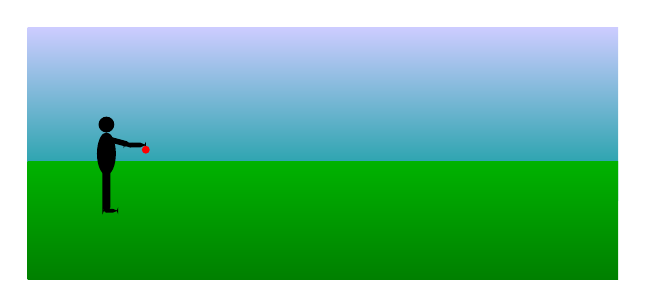
\begin{tikzpicture}%[scale=0.5]
    %  Ciel
  \shade[bottom color=cyan!60!black, top color=blue!20!white] (0,0) rectangle (7.5,2.2);
    %  Sol
  \shade[bottom color=green!50!black, top color=green!70!black] (0,0.5) rectangle (7.5,-1);
    %  Mare
 % \shade[bottom color=blue!50!white, top color=cyan!60!black] (3.7,-0.15) ellipse (2.5 and 0.3);
    %  Arbre
 % \pic at (2,2)    {arbre};

    %  Personnage
  \begin{scope}[xshift=1 cm,yshift=0.6 cm]
    % corps et tête
 \fill [black] (0,0)ellipse(0.12 and 0.27);
 \fill [black](0,0.37)circle(0.1);
    % jambe et pieds
 \fill [rounded corners=2pt] (0.05,-0.15)rectangle(-0.05,-0.75);
 \fill [rounded corners=2pt] (0.15,-0.7)rectangle(-0.05,-0.75);
    % bras
 \fill [rounded corners=2pt, rotate=-15] (-0.1,0.22)rectangle(0.28,0.15);
 \fill [rounded corners=2pt] (0.22,0.08)rectangle(0.5,0.14);
   % Balle
 \fill[red] (0.5,0.05) circle(0.05);
  \end{scope}

\end{tikzpicture}

%%%%%%%%%%%%%%%%%%%%%%%%%%%%%%%%%%%%%%%%%%%%%%%%%%%%%%%%%%%%%%%%%%%%%%%%%%%%%%%%

\texttt{FIGURE}
\end{center}
%Le champ électrique $\overrightarrow{E}$ exerce une force $\overrightarrow{F}_{\overrightarrow{E}/Q_2}$ sur la charge électrique $Q_2$
%\end{minipage}

%\subsection{Champ magnétique}

%%%%%%%%%%%%%%%%%%%%%%%%%%%%%%%%%%%%%%%%%%%%%%%%%%%%%%%%%%%%%%%%%%%%%%%%%%%%
